% !TeX root = ../../thesis.tex
\chapter{Materials and methods}
\label{ch:methodology}

% \section{Genomic sequence data}
%
% For both Hepatitis B and Lassa analyses our genomic sequence came from a variety of sources.
% Both analyses were comprised of a majority of sequences pulled directly from publically available sequence databses.
% Additionally, both analyses include a subset of novel sequences generated by their respective study groups that have not yet been released publically.

\section{Bayesian phylogeographic inference of HBV}

\subsection{Genomic sequence data}
We analyze a total of 1,590 Hepatitis B virus genomes. %GB: how was this amount decided upon? Are these considered to be full/complete genomes?
These genomes were divided into three datasets based on their HBV subgenotype, such that we had 587 HBV-A genomes, 769 HBV-D genomes, and 234 HBV-E genomes.
Of these, the vast majority (total 1,466: 540 HBV-A, 765 HBV-D, 170 HBV-E) were provided by collaborators following a query of the GenBank sequence database. %GB: this begs the question where the other ones came from; you can mention this information and prepare for questions (rudimentary ones) on how these data were generated, i.e. which technology (Illumina, MinION, ...).
In order to investigate temporal signal in these HBV data sets, we perform additional analyses by including -- for two of the subgenotypes -- recently published `ancient' genomes isolated from mummies ranging in age from 450 years old to 4,500 years old \cite{muhlemann, ross}. %GB: I would make sure to mention `ancient' as this will tie in nicely with your explanation of measurably evolving populations in the introduction, where you should talk about `ancient DNA' data sets and mention Beth Shapiro's Science paper on bison populations.
The underlying assumption is that these genomes may help to improve temporal signal in the HBV datasets, as typically remarkably little signal is present in such data.
We will assess whether the addition of these ancient samples allows to infer approximate timing windows of historical events.

\subsection{Preprocessing}

Prior to Bayesian inference, we estimated unrooted maximum likelihood phylogenetic trees using IQ-TREE. %GB: citation?
These maximum likelihood trees were used to perform temporal signal analysis using TempEST, %GB: citation?
allowing us to remove sequences that showed incongruent temporal signal patterns.
%GB: I would talk more about TempEst and what it tries to do; the next two sequences are technically results.
The resulting dataset comprised 583 sequences of HBV-A genotype viruses, 764 HBV-D sequences, and 234 sequences HBV-E genotype viruses.
With the inclusion of ancient genomes, the final HBV-A and HBV-D datasets included 587 and 769 total taxa, respectively.

\subsection{Phylogenetic modeling}

We inferred phylogenetic trees for each of our three datasets by performing Bayesian inference using MCMC as implemented in BEAST1.10. %GB: citation?
For all datasets we used the same model specification as detailed below.
Branch rates were inferred under an uncorrelated relaxed molecular clock model assuming an underlying lognormal distribution, allowing us accommodate evolutionary rate variation across the branches of the phylogeny.
Following unsuccessful modeling of demographic history under a Bayesian skygrid model, we used a constant demographic model as a tree model. %GB: I don't mind this sentence, but it can lead to questions
To accommodate the impact of the overlapping regions in the HBV genome on the substitution process of each codon position, we assumed an HKY substitution model without codon partitioning, accommodating among-site rate heterogeneity through a discretized gamma distribution. %GB: citation?
We performed at least three independent replicates of our MCMC analysis to ensure proper convergence, with each replicate running for 500 million iterations and subsampling every 10,000th iteration. %GB: make sure to be specific as to which approaches help with convergence and which help with mixing, as these are entirely different aspects
We assumed default priors in BEAST for all parameters these analyses except for lognormal substitution rate ($X \sim Lognormal(-11.3474,1.22)$), %GB: I would avoid this type of math notation (it's also not defined what X is) and simply write down the mean and standard deviation (and mention the correct scale)
which was derived from the HBV substitution rate estimated by the researchers who generated the ancient genomes \cite{muhlemann}.
To speed up likelihood computations we used the BEAGLE 3 high-performance computational library.
MCMC chains were run for 500 million iterations and were sampled every 25,000th state.
For each subtype, multiple replicates were run in parallel using different starting seeds to ensure proper convergence and statistical mixing, and a single combined posterior distribution was formed from all replicates, removing an appropriate proportion (at least 10\%) of each chain as burn-in.
From this combined posterior distribution, 1,000 trees were sampled and used to perform subsequent Bayesian phylogeographic reconstruction in BEAST using empirical tree distributions. %GB: it wasn't discussed why this step was taken I think


\subsection{Phylogeographic modeling}

Employing the collected empirical tree distributions, we estimated the spatial diffusion dynamics using a Bayesian phylogeographic approach in which the locations are treated as discrete traits, and allowed for different migration rates to and from each location.
This approach conditioned on the geographic locations recorded at the tips of the trees and models the transition history among those locations as a continuous-time Markov chain (CTMC) process to infer the unobserved locations at the internal nodes of each tree.
For these reconstructions, MCMC chains were run for 10 million iterations and sampled every 10,000th state.
Maximum clade credibility (MCC) trees were summarized using TreeAnnotator v1.10 (cite BEAST 1.10) and the resulting trees were visualized in FigTree v1.4.3.
The links between locations that contribute significantly to explaining the migration history were identified using a Bayesian stochastic search variable selection (BSSVS) procedure, and SpreaD3 %GB: citation?
was used to calculate the Bayes factor (BF) support for these links.
We also estimated the expected number of location state transitions in the ancestral history conditional on the data observed at the tree tips using ``Markov jump" counts, providing a quantitative measure of asymmetry in viral flow between regions.
Since the data consist of a heterogeneous number of sequences for each location which show strong sampling bias between individual countries that can strongly impact the outcome of a discrete phylogeography study.
To mitigate this issue, we opted to group sequences into continental regions, aiming to contain a number of sequences of the same order of magnitude where possible: Africa, the Americas, East South Asia, Europe, and West Central Asia. %GB: I would not go into detail here, but make a general statement and refer to the results section for the different options/groupings we considered
We note that for data set E, no samples from East South Asia nor West Central Asia were available.




\section{Lassa phylogenetics and online inference}

\subsection{Adaptable bipartite build framework}

Lassa virus (LASV) proves to be a particularly difficult virus to preprocess for the purposes of phylogenetic inference.
In particular, generating an accurate and useful alignment can be very challenging with LASV due to its high sequence variability.
The challenges from this variability are compounded, as they need to be accounted for both across Lassa's two genomic segments, but also for the two genes on each of the segments, which need to be aligned to each other to provide meaningful results during phylogenetic analysis. %GB: this makes it sounds as though we need to introduce the genome structure of LASV? But probably do this in the results section and refer to it from here.
To handle these challenges, we divide our adaptable processing framework into two steps, one for alignment generation, and one for build parameterization and specification.

\subsubsection{Snakemake for build management}

For both of these steps, we employ the use of Snakemake \cite{snakemake}, a flexible workflow management system designed to be used with the Python programming language, to manage build specifications and easily perform online Bayesian inference.
We use this as an alternative to the traditional methods of workflow management---most commonly simple shell scripts or repeated use of command line tools.
The use of Snakemake in our build pipelines affords us three major advantages over previous methods of build management: increased build reproducibility, easy parameterization, and robust error management.

A pipeline is broken into its component steps as a series of ``rules"---each encapsulating a single command line directive---that can be parameterized by a single configuration file.
Each rule is defined in terms of its expected input and output as filenames; each rule also specifies a particular directive that should generate the outputs from the input.
For example, one could specify a rule, \texttt{count\_lines}, whose goal was to apply the \texttt{wc -l} command line utility to an \texttt{input.txt} file and generate an \texttt{output.txt} file.
At runtime Snakemake would check that \texttt{output.txt} did not already exist on the filesystem---an important check that prevents costly recomputation.
Next, Snakemake would check if \texttt{input.txt} existed on the filesystem, yielding an error if the file were not present.
Snakemake would then apply the specified command line utility.
Finally, Snakemake would check that \texttt{output.txt} existed in the filesystem, throwing an error if the expected file were not present.
Importantly, Snakemake allows us to generalize these steps so that one's input is determined as a function of the previous step's output, and to apply dynamic changes to the workflow according to user specified variables.
This combination of rules being ``strung" together, plus filesystem checks to determine presence or absence of input and output files, affords us the opportunity to update builds quickly and without performing unnecessary recomputations.

Because each command is centralized into the Snakemake workflow, exact reproduction of past analyses becomes trivial.
Indeed, reproduction of past analyses with minor alterations (e.g. a slightly updated dataset, different MCMC chain length) also becomes trivial, as all parameters are saved in a single configuration JSON file, rather than memorized or stored in shell history.
This is of particular importance because it allows for easy specification of updated builds without running the risk of losing previously performed analyses due to filesystem overwrites (a concern when using shell scripting or command line copy/pasting).
It also ensures that all build parameters and commands that are not explicitly modified by the user are kept constant, ensuring consistency between builds.

\subsubsection{Alignment generation}

Our initial Lassa analyses began with genomes gathered from GenBank via API query and from previously unpublished genomes from 2019 seasonal outbreaks in Nigeria provided by collaborators (671 L segments, 795 S segments). %GB: cite Liana's 2019 Science paper? Or not applicable here?
Midway through the analysis period we received incoming data updates from collaborators in Nigeria, increasing our dataset sizes to respectively 698 L segments and 826 S segments.
Data from collaborators were provided to us as Microsoft Excel spreadsheets containing both sequences and metadata, necessitating a preprocessing pipeline that could collate new genomes with those generated by GenBank query.
For each sequence, its genotype was determined according to BLAST search.
Genotype-gene alignments were then built using MAFFT and concatenated ``vertically" across genotypes. %GB: citation?
Finally, alignments were concatenated ``horizontally" between the two genes for each segment, padded with \textit{N} characters to allow for variations in length and to buffer between genes.
This process is illustrated in Figure~\ref{fig:alignment_dag}.

%GB: so for properly understanding this figure, we should probably describe the LASV genome as otherwise this figure is too difficult to understand.
\begin{figure}[ht]
  \centering
  \medskip
  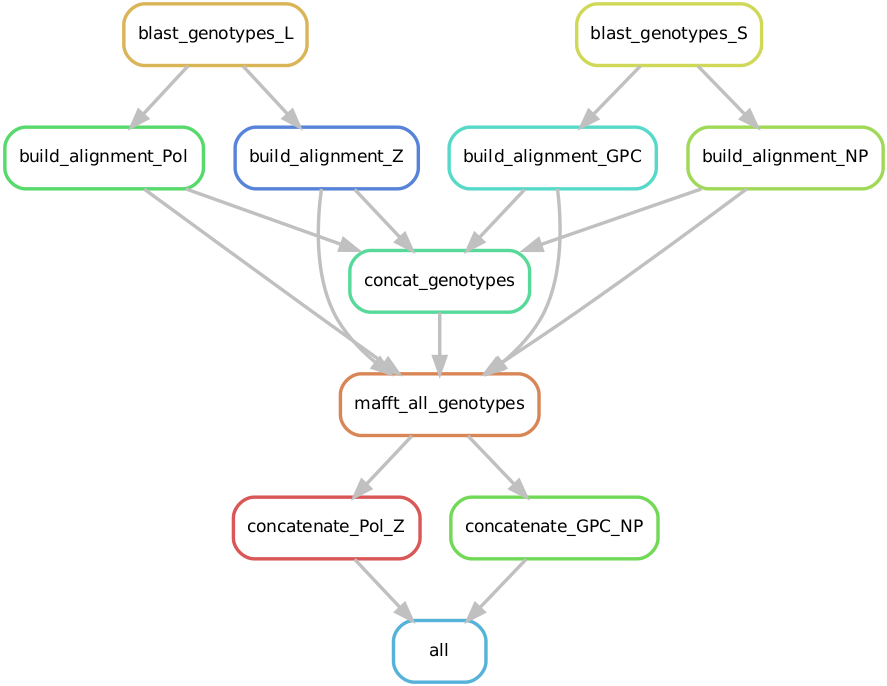
\includegraphics[width=.9\textwidth]{alignment_dag}
  \caption[Lassa alignment pipeline]{A directed acyclic graph (DAG) representing the pipeline by which we generate Lassa virus alignments. We first use BLAST on each segment to determine its genotype. We then build gene-specific alignments for each genotype, and concatenate the results ``vertically"---i.e. all alignment files are combined into one. Then, we update the alignments such that all genotypes are as well aligned with each other as possible. Finally, we combine each gene ``horizontally" within each segment---i.e. for each segment and each strain there is a single sequence in the alignment---such that the final result are two final alignment files, one for each genome.}
  \label{fig:alignment_dag}
\end{figure}

\subsubsection{MCMC build specification}

For our Lassa analyses, we created a Snakemake pipeline similar in form to that used for preprocessing.
This pipeline (Fig.~\ref{fig:workflow_dag}) took the output alignments described above as its primary input.
From each, we generated BEAST XML files.
We use a Bayesian skygrid demographic models for our analyses---though the pipeline is parameterized to easily accommodate both constant population size and Bayesian Skyride demographic models.
Our skygrid inference used a Hamiltonian Monte Carlo (HMC) operator to allow efficient transition of population size state space. %GB: citation?
We assumed an HKY substitution model with codon partitioning for each gene, accommodating among-site rate heterogeneity through a discretized gamma distribution.
We otherwise assume default BEAST values for operators and priors.
The MCMC chain length, logging frequency, and number of parallel replicates were parameterized dynamically though Snakemake, however for the results we present we ran a single chain for $5\times10^7$ iterations, logging every 15,000th state.

For each segment, after its parallel BEAST replicates were completed, we remove burnin from each log (minimum 10\%), and concatenate logs to form one joint posterior sample set.
We perform an identical process for posterior trees.
We use these combined parameter and tree distributions to generate MCC trees for each segment.

\begin{figure}[ht]
  \centering
  \medskip
  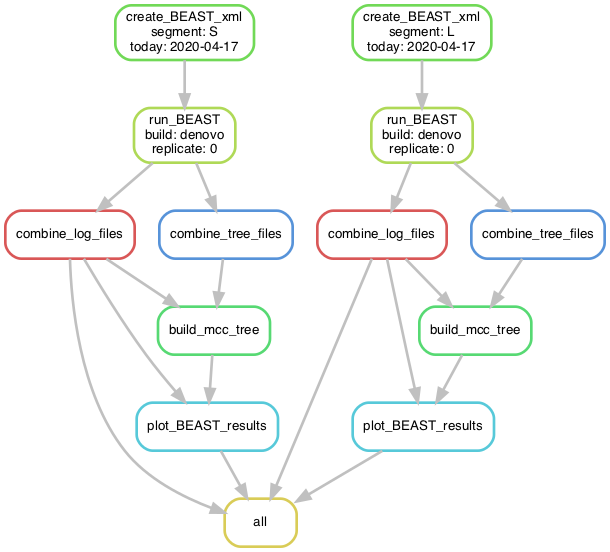
\includegraphics[width=.9\textwidth]{workflow_dag}
  \caption[Lassa phylogenetics pipeline]{A directed acyclic graph (DAG) representing the pipeline by which we perform Lassa virus phylogenetic inference. We perform identical workflows for each genomic segment. After BEAST XMLs are generated and run, we remove burnin and analyze the results of combined parameter and tree distributions.}
  \label{fig:workflow_dag}
\end{figure}

%%%%%%%%%%%%%%%%%%%%%%%%%%%%%%%%%%%%%%%%%%%%%%%%%%
% Keep the following \cleardoublepage at the end of this file,
% otherwise \includeonly includes empty pages.
\cleardoublepage

% vim: tw=70 nocindent expandtab foldmethod=marker foldmarker={{{}{,}{}}}
